\onehalfspacing
\section{Đề số 11}
\graphicspath{{./img/}}
\begin{bt} 
    \hfill
	\begin{enumerate}[a.]
		\item Tính giá trị của biểu thức: $A=\frac{4}{9}:\left(\frac{1}{15}-\frac{2}{3}\right)+\frac{4}{9}:\left(\frac{1}{11}-\frac{5}{22}\right)$
        \item Tìm $x$, biết: $\left(-1 \frac{3}{5}+x\right): \frac{12}{13}=2 \frac{1}{6}$
        \item Tính giá trị của biểu thức $M=21 x^2 y+4 x y^2$ với $x$, $y$ thoả mãn:
        $$
        (x-2)^4+(2 y-1)^{2014} \leq 0
        $$
	\end{enumerate}
	\loigiai{
		\begin{enumerate}
			\item A = $\frac{4}{9}: \frac{-3}{5}+\frac{4}{9}: \frac{-3}{22}=\frac{4}{9} \cdot\left(\frac{-5}{3}+\frac{-22}{3}\right)=-4$
			\item Ta có: $\left(-1 \frac{3}{5}+x\right): \frac{12}{13}=2 \frac{1}{6}$\\ 
			$\Leftrightarrow-1 \frac{3}{5}+x=\frac{13}{6} \cdot \frac{12}{13}\\ 
			\Leftrightarrow x=3 \frac{3}{5}$
			\item Vì $(x-2)^4 \geq 0$; $(2 y-1)^{2014} \geq 0$ với mọi $x$, y nên $(x-2)^4+(2 y-1)^{2014} \geq 0$.\\ Mà $(x-2)^4+(2 y-1)^{2014} \leq 0$\\
			Suy ra $(x-2)^4=0$ và $(2 \mathrm{y}-1)^{2014}=0$ suy ra $x=2, y=\frac{1}{2}$\\
			Khi đó $M=44$.
		\end{enumerate}
	} 
\end{bt}

\begin{bt}
	\hfill
	\begin{enumerate}[a.]
		\item Tìm các số $\mathrm{x}, \mathrm{y}, \mathrm{z}$ biết: $\frac{x}{3}=\frac{y}{4} ; \quad \frac{y}{6}=\frac{z}{8} \quad$ và $2 x+y-z=-14$.
        \item Tìm $x$, biết: $(x-2)\left(x+\frac{2}{3}\right)>0$.
        \item Tìm số nguyên $x$, biết rằng: $\frac{3}{7} \cdot 15 \frac{1}{3}+\frac{3}{7} \cdot 5 \frac{2}{5} \leq x \leq\left(3 \frac{1}{2}: 7-6 \frac{1}{2}\right) \cdot\left(-2 \frac{1}{3}\right)$
	\end{enumerate}
	\loigiai{
		\begin{enumerate}
			\item Từ $\frac{x}{3}=\frac{y}{4} ; \quad \frac{y}{6}=\frac{z}{8} \Rightarrow \frac{x}{9}=\frac{y}{12}=\frac{z}{16}$\\
			Vậy: $\frac{x}{9}=\frac{y}{12}=\frac{z}{16}=\frac{2 x}{18}=\frac{y}{12}=\frac{z}{16}=\frac{2 x+y-z}{18+12-16}=\frac{-14}{14}=-1$\\ 
			Suy ra $x=-9 ; y=-12 ; z=-16$
			\item Từ $(x-2)\left(x+\frac{2}{3}\right)>0$ suy ra $x-2$ và $x+\frac{2}{3}$ cùng dấu.\\ 
			Dễ thấy $x-2<x+\frac{2}{3}$ nên ta có:\\
			* $x-2$ và $x+\frac{2}{3}$ cùng dương $\Leftrightarrow x-2>0 \Leftrightarrow x>2$.\\
			* $x-2$ và $x+\frac{2}{3}$ cùng âm $\Leftrightarrow x+\frac{2}{3}<0 \Leftrightarrow x<-\frac{2}{3}$\\
			Vậy $x>2$ hoặc $x<-\frac{2}{3}$.
			\item Ta có $\frac{3}{7} \cdot 15 \frac{1}{3}+\frac{3}{7} \cdot 5 \frac{2}{5}=\frac{3}{7} \cdot\left(15 \frac{1}{3}+5 \frac{2}{5}\right)=8 \frac{31}{35} \left(3 \frac{1}{2}: 7-6 \frac{1}{2}\right) \cdot\left(-2 \frac{1}{3}\right)=14$\\
			Do đó: $8 \frac{31}{35} \leq x \leq 14$, vì x nguyên nên $x \in\{9 ; 10 ; 11 ; 12 ; 13 ; 14\}$
		\end{enumerate}
	} 
\end{bt}

\begin{bt}
	\hfill
	\begin{enumerate}[a.]
		\item Tính giá trị của biểu thức $\mathrm{M}=4 \mathrm{x}+4 \mathrm{y}+21 \mathrm{xy}(\mathrm{x}+\mathrm{y})+7\left(\mathrm{x}^3 \mathrm{y}^2+\mathrm{x}^2 \mathrm{y}^3\right)+2014$, biết $\mathrm{x}+\mathrm{y}=0$.
        \item Cho đa thức $p(x)=a x^3+b x^2+c x+d$, với $a, b, c, d$ là các hệ số nguyên. Biết rằng, $\mathrm{p}(\mathrm{x}) \vdots 5$ với mọi $\mathrm{x}$ nguyên. Chứng minh rằng $\mathrm{a}, \mathrm{b}, \mathrm{c}, \mathrm{d}$ đều chia hết cho 5 .
        \item Cho $A=1+\frac{1}{2}+\frac{1}{3}+\frac{1}{4}+\ldots+\frac{1}{4026}, B=1+\frac{1}{3}+\frac{1}{5}+\frac{1}{7}+\ldots+\frac{1}{4025}$. So sánh $\frac{A}{B}$ với $1 \frac{2013}{2014}$.
	\end{enumerate}
	\loigiai{
		\begin{enumerate}
			\item $M=4(x+y)+21 x y(x+y)+7 x^2 y^2(x+y)+2014=2014$
				(Vì x+y=0)
			\item Vì $\mathrm{p}(\mathrm{x}) \vdots 5$ với mọi $x$ nguyên nên $\mathrm{p}(0)=\mathrm{d} \vdots 5$.\\
			$\mathrm{p}(1)=\mathrm{a}+\mathrm{b}+\mathrm{c}+\mathrm{d}: 5$ (1)\\
			$p(-1)=-a+b-c+d: 5$ (2)\\
			Từ (1) và (2) suy ra : $2(\mathrm{~b}+\mathrm{d}) \vdots 5$ và $2(\mathrm{a}+\mathrm{c}) \vdots 5$.\\
			Vì $2(b+d) \vdots 5$, mà $(2,5)=1$ nên $b+d \vdots 5$ suy ra $b \vdots 5$.\\
			$p(2)=8 a+4 b+2 c+d \vdots 5$ mà $d \vdots 5 ; b \vdots 5$. nên $8 a+2 c \vdots 5$,
			kết hợp với $2(a+c) \vdots 5$ suy ra $6 a \vdots 5$ suy ra $a \vdots 5$ vì $(6,5)=1$. từ đó $\mathrm{c} \vdots 5$.\\
			Vậy a, b, c, d đều chia hết cho 5 .
			\item Đặt $C=A-B=\frac{1}{2}+\frac{1}{4}+\frac{1}{6}+\ldots+\frac{1}{4026}$\\
			Ta có $B=1+\frac{1}{3}+\frac{1}{5}+\frac{1}{7}+\ldots+\frac{1}{4025}>1+\frac{1}{4}+\frac{1}{6}+\ldots+\frac{1}{4026}=\frac{1}{2}+C$ (1)\\ 
			Lại có:
            $$
            \begin{aligned}
            & \frac{2013}{2}=\underbrace{\frac{1}{2}+\frac{1}{2}+\frac{1}{2}+\ldots+\frac{1}{2}}_{2013 \text { sohang }}>\frac{1}{2}+\frac{1}{4}+\frac{1}{6}+\ldots+\frac{1}{4026}=C \\
            & \Rightarrow \frac{1}{2}>\frac{C}{2013} (2)\\
            &
            \end{aligned}
            $$
            Từ (1) và (2) suy ra $B>\frac{C}{2013}+C \Rightarrow 2013 B>2014 C$\\
            Do đó: $\frac{C}{B}<\frac{2013}{2014} \Rightarrow \frac{C+B}{B}<1 \frac{2013}{2014} \Rightarrow \frac{A}{B}<1 \frac{2013}{2014}$
		\end{enumerate}
	} 
\end{bt}

\begin{bt}
	Cho tam giác $A B C$ cân tại $A$. Trên cạnh $B C$ lấy điểm $D$ ( $D$ khác $B, C$ ). Trên tia đối của tia $C B$, lấy điểm $\mathrm{E}$ sao cho $\mathrm{CE}=\mathrm{BD}$. Đường vuông góc với $\mathrm{BC}$ kẻ từ $\mathrm{D}$ cắt $\mathrm{BA}$ tại $\mathrm{M}$. Đường vuông góc với $\mathrm{BC}$ kẻ từ $\mathrm{E}$ cắt tia $\mathrm{AC}$ tại $\mathrm{N}$. $\mathrm{MN}$ cắt $\mathrm{BC}$ tại $\mathrm{I}$.
	\begin{enumerate}[a.]
		\item Chứng minh rằng: $\mathrm{DM}=\mathrm{EN}$.
        \item Chứng minh rằng $\mathrm{IM}=\mathrm{IN} ; \mathrm{BC}<\mathrm{MN}$.
        \item Gọi $\mathrm{O}$ là giao của đường phân giác góc $\mathrm{A}$ và đường thẳng vuông góc với $\mathrm{MN}$ tại $\mathrm{I}$. Chứng minh rằng: $\triangle B M O=\triangle C N O$. Từ đó suy ra điểm $\mathrm{O}$ cố định.
	\end{enumerate}
	\loigiai{
		$$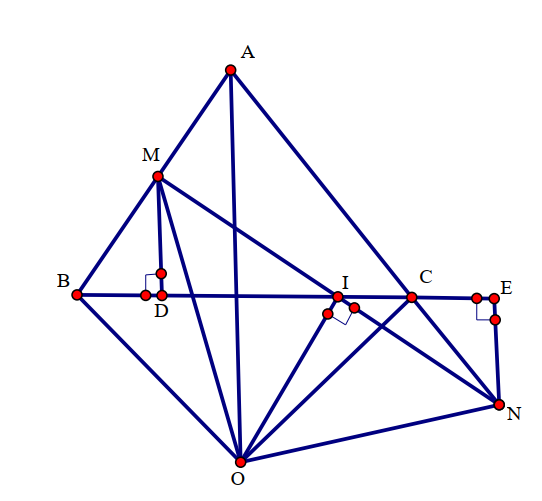
\includegraphics[width=0.55\textwidth]{11-4-lg.png}$$
		\begin{enumerate}
			\item Tam giác $\mathrm{ABC}$ cân tại A nên $A B C=A C B ; \quad N C E=A C B$; (đối đỉnh)\\
			Do đó: $\triangle M D B=\triangle N E C($ g.c.g) $\Rightarrow D M=E N$
			\item Ta có $\triangle M D I=\triangle N E I$ (g.c.g) $\Rightarrow M I=N I$\\
			Vì $\mathrm{BD}=\mathrm{CE}$ nên $\mathrm{BC}=\mathrm{DE}$.\\
			Lại có $\mathrm{DI}<\mathrm{MI}$, IE $<\mathrm{IN}$ nên $\mathrm{DE}=\mathrm{DI}+\mathrm{IE}<\mathrm{MI}+\mathrm{IN}=\mathrm{MN}$\\
			Suy ra $B C<M N$.
			\item Ta chứng minh được:\\
			$\triangle A B O=\triangle A C O(\text { c.g.c }) \Rightarrow O C=O B, A B O=A C O . \\
			\triangle M I O=\triangle N I O(\text { c.g.c }) \Rightarrow O M=O N .$\\
			Lại có: $\mathrm{BM}=\mathrm{CN}$, do đó $\triangle B M O=\triangle C N O$ (c.c.c)\\ 
			$\Rightarrow M B O=N C O \text {, Mà: } M B O=A C O \text { suy ra } N C O=A C O \text {, }$\\
            mà đây là hai góc kề bù nên $\mathrm{CO} \perp \mathrm{AN}$.\\
            Vì tam giác $\mathrm{ABC}$ cho trước, $\mathrm{O}$ là giao của phân giác góc $\mathrm{A}$ và đường vuông góc với $\mathrm{AC}$ tại C nên $O$ cố định.
		\end{enumerate}
	}
\end{bt}

\begin{bt}
Cho tam giác $\mathrm{ABC}$ cân tại $\mathrm{A}$. Trên đường trung tuyến $\mathrm{BD}$ lấy điểm $\mathrm{E}$ sao cho $D A E=A B D$ (E nằm giữa $\mathrm{B}$ và $\mathrm{D}$ ). Chứng minh rằng $D A E=E C B$.
\loigiai{
	$$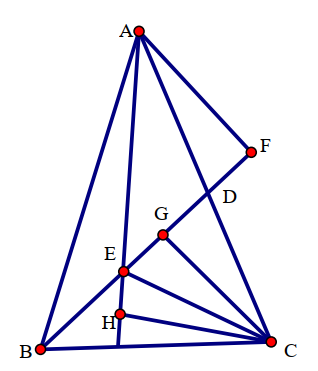
\includegraphics[width=0.4\textwidth]{11-5-lg.png}$$
	Vẽ AF vuông góc $\mathrm{BD}, \mathrm{CG}$ vuông góc $\mathrm{BD}, \mathrm{CH}$ vuông góc với $\mathrm{AE}$.\\ 
	Ta có $\triangle A B F=\triangle C A H$ (cạnh huỳen - góc nhon). Suy ra: $\mathrm{AF}=\mathrm{CH}$. $\triangle A D F=\triangle C D G(c h-g n)$ suy ra $A F=C G$.\\
    Từ đó ta có $\mathrm{CH}=\mathrm{CG}$.
    $\triangle C E H=\triangle C E G(c h-c g v) \Rightarrow C E H=C E G ;$
    Mà $C E G=E B C+E C B ; C E H=E A C+E C A$;\\
    Do đó: $E B C+E C B=E A C+E C A ;(1)$\\
    Mặt khác: $E B A+E B C=E C B+E C A ;(2)$\\
    Lấy (1) trừ (2) theo vế ta có:\\
    $E C B-E B A=E A C-E C B=E B A-E C B \\
    \Rightarrow E B A=E C B$\\
    Mà $D A E=A B D$ nên $D A E=E C B$.
}
\end{bt}